% Manual de conexión y uso del gemelo digital del brazo XK-JS1-1 (II-2026)
% Compilar desde esta carpeta:  pdflatex manual_gemelo_digital.tex (dos veces)
\documentclass[a4paper,11pt]{article}
\usepackage{geometry}
\geometry{letterpaper, margin=2.2cm}
\usepackage[spanish, es-nodecimaldot, mexico]{babel}
\usepackage[utf8]{inputenc}
\usepackage[T1]{fontenc}
\usepackage{lmodern}
\usepackage[table]{xcolor}
\definecolor{naranja}{RGB}{194,98,12}
\definecolor{rojo}{RGB}{192,57,43}
\definecolor{verde}{RGB}{30,120,70}
\definecolor{gris}{RGB}{242,242,242}
\usepackage{booktabs,longtable,array,tabularx}
\usepackage{graphicx}
\usepackage{float}
\usepackage{caption}
\captionsetup{font=small, labelfont=bf}
\usepackage{tikz}
\usetikzlibrary{positioning,arrows.meta,fit,shapes.geometric}
\usepackage{enumitem}
\setlist{itemsep=2pt}
\usepackage{listings}
\lstset{basicstyle=\ttfamily\small, frame=single, backgroundcolor=\color{gris}, breaklines=true,
  columns=fullflexible, keepspaces=true, extendedchars=true,
  literate={á}{{\'a}}1 {é}{{\'e}}1 {í}{{\'i}}1 {ó}{{\'o}}1 {ú}{{\'u}}1 {ñ}{{\~n}}1 {…}{{...}}3}
\usepackage{hyperref}
\hypersetup{colorlinks=true, linkcolor=naranja, urlcolor=naranja}
\usepackage{fancyhdr}
\pagestyle{fancy}
\fancyhf{}
\lhead{\small Gemelo digital del brazo XK-JS1-1}
\rhead{\small Manual de conexión y uso}
\cfoot{\small \thepage}
\newcommand{\codigo}[1]{\texttt{#1}}
\newcommand{\aviso}[1]{\par\smallskip\noindent\colorbox{rojo!10}{\parbox{\dimexpr\linewidth-2\fboxsep}{\textbf{\color{rojo}Atención.} #1}}\par\smallskip}
\newcommand{\nota}[1]{\par\smallskip\noindent\colorbox{gris}{\parbox{\dimexpr\linewidth-2\fboxsep}{#1}}\par\smallskip}
% marcas numeradas sobre las capturas
\tikzset{marca/.style={circle, fill=naranja, text=white, font=\bfseries\footnotesize, inner sep=1.4pt, minimum size=4.6mm, draw=white, line width=0.8pt}}
\DeclareRobustCommand{\num}[1]{\tikz[baseline=-0.7ex]\node[marca]{#1};}
% \captura{ancho}{archivo}{marcas en coordenadas 0-1 desde la esquina inferior izquierda}
\newcommand{\captura}[3]{%
  \begin{tikzpicture}
  \node[anchor=south west, inner sep=0, draw=black!25] (img) {\includegraphics[width=#1]{#2}};
  \begin{scope}[x={(img.south east)}, y={(img.north west)}]
  #3
  \end{scope}
  \end{tikzpicture}}

\title{\textbf{Gemelo digital del brazo XK-JS1-1}\\[4pt]\large Manual de conexión y uso: app local, acceso remoto y usuarios}
\author{ETN-902 / ETN-1034 / ETN-1000 · UMSA · II-2026}
\date{28 de octubre de 2026}

\begin{document}
\maketitle
\thispagestyle{fancy}

\tableofcontents
\newpage

% =====================================================================
\section{Qué es}

La app \codigo{gemelo\_brazo.py} une tres cosas:
\begin{enumerate}
\item el PLC S7-200 del brazo, a través del cable USB-PPI (protocolo PPI, el mismo de STEP 7-Micro/WIN);
\item el visor 3D del proyecto, que dibuja el brazo con la cinemática del modelo;
\item un pequeño servidor web por el que la página lee el estado del brazo y, si se permite, le da órdenes.
\end{enumerate}

Hay tres formas de ver el gemelo:

\begin{center}
\begin{tikzpicture}[caja/.style={draw, rounded corners, fill=gris, minimum height=12mm, text width=30mm, align=center, font=\small},
  >={Stealth}, node distance=8mm and 16mm]
\node[caja] (plc) {PLC S7-200\\CPU 224 CN};
\node[caja, right=of plc] (pc) {\textbf{PC del laboratorio}\\app \codigo{gemelo\_brazo.py}};
\node[caja, right=of pc, fill=naranja!12] (router) {router o Wi-Fi\\del laboratorio};
\node[caja, below=of pc, fill=white] (local) {ventana de la app\\\codigo{localhost:8050}};
\node[caja, below=of router, fill=white] (cel) {celulares y PC\\usuario y contraseña};
\node[caja, below=of plc, fill=white, draw=black!40] (pub) {página pública\\solo simulación};
\draw[<->, thick] (plc) -- node[above, font=\scriptsize]{USB-PPI} (pc);
\draw[<->, thick] (pc) -- node[above, font=\scriptsize]{red local} (router);
\draw[<->, thick] (router) -- node[right, font=\scriptsize]{HTTPS :8443} (cel);
\draw[<->] (pc) -- (local);
\node[draw=black!30, dashed, rounded corners, inner sep=2.5mm, fit=(plc)(pc)(local)] {};
\node[font=\scriptsize, below=1mm of pub] {internet: no llega al brazo};
\end{tikzpicture}
\end{center}

\begin{center}\small
\begin{tabularx}{\linewidth}{>{\raggedright}p{3.6cm} >{\raggedright}X >{\raggedright\arraybackslash}X}
\toprule
\textbf{Dónde} & \textbf{Quién} & \textbf{Qué puede hacer}\\
\midrule
\textbf{App local} (PC con el cable) & quien está en la planta; sin contraseña & ver, mover, calibrar, dar paro\\
\textbf{Acceso remoto} (misma red) & usuarios creados en la PC del laboratorio & observador: ver; operador: ver, tomar el mando, mover, dar paro\\
\textbf{Página pública} (internet) & cualquiera & simular el brazo; no manda el brazo real\\
\bottomrule
\end{tabularx}
\end{center}

La app reconoce sola el programa que tiene el PLC y se adapta:

\begin{center}\small
\begin{tabularx}{\linewidth}{>{\raggedright}p{4.2cm} >{\raggedright}X >{\raggedright\arraybackslash}X}
\toprule
\textbf{Programa en el PLC} & \textbf{Qué muestra la página} & \textbf{Qué se puede mandar}\\
\midrule
\codigo{plc/brazo\_gemelo} (perfil \emph{gemelo}) & Brazo en vivo con la posición \textbf{contada en el PLC} & Homing, mover a cualquier posición (articular o cartesiana), secuencias grabadas, garra, velocidad\\
Programa anterior de secuencias (perfil \emph{cargado}) & Brazo en vivo con la posición \textbf{estimada} a partir de los trenes de pulsos & Iniciar (homing o secuencia siguiente), Detener, Paro de emergencia, Rearmar\\
Otro programa (perfil \emph{monitor}) & Entradas, salidas y posición estimada & Nada\\
\bottomrule
\end{tabularx}
\end{center}

% =====================================================================
\section{Seguridad}
\begin{itemize}
\item Mientras alguien tenga el mando (en la PC o en un celular), una persona debe estar junto a la \textbf{seta de emergencia} del tablero. El paro de la página no la reemplaza.
\item El \textbf{selector del panel (I0.5)} decide quién manda: en \emph{manual} solo el panel; en \emph{automático} la PC o un operador remoto.
\item El mando desde la página está \textbf{deshabilitado} al arrancar. Para habilitarlo hay que marcar la casilla y confirmar. Un solo operador tiene el mando a la vez.
\item Si la app, la página o el cable fallan, el PLC se detiene solo: el programa del gemelo tiene un watchdog de 2 s y el programa anterior borra las órdenes de la PC a los 5 s.
\item La app solo escribe en zonas fijas de la memoria V (\codigo{VB1100-{}-VB1119} con el programa del gemelo; \codigo{VB100} y \codigo{VB104} con el anterior). Cualquier otra escritura se rechaza antes de salir por el cable.
\item Cada ingreso, cada orden aceptada y cada orden rechazada quedan en \codigo{registro\_gemelo.log}, con hora y usuario.
\item Antes de mover, hacer siempre el \textbf{homing}: sin él la posición del modelo no coincide con la real.
\end{itemize}

% =====================================================================
\section{Requisitos}
\begin{itemize}
\item PC con Linux (probado en Ubuntu) y \textbf{Python 3.8 o superior}. No hay que instalar paquetes: la app usa solo la biblioteca estándar. Para la ventana propia se usa GTK y WebKit, que ya trae Ubuntu.
\item Cable \textbf{USB-PPI} (el del laboratorio aparece como \codigo{CH340 serial converter}, \codigo{/dev/ttyUSB0}).
\item El usuario de Linux debe estar en el grupo \codigo{dialout} (comprobar con \codigo{groups}). Si no está: \codigo{sudo usermod -aG dialout \$USER} y volver a iniciar sesión.
\item Para el acceso remoto: un router o Wi-Fi al que estén conectados la PC del laboratorio y los celulares.
\end{itemize}
\nota{\textbf{Alternativa al cable USB-PPI (por comprobar).} El puerto del S7-200 es RS-485, así que un convertidor USB--RS485 con cambio de dirección automático debería servir: A(+) al pin 3 del DB9, B($-$) al pin 8 y GND al pin 5 (si no responde, invertir A y B). Conviene uno con aislamiento galvánico. Se indica el puerto con \codigo{-{}-puerto /dev/ttyUSB1} si Linux le da otro nombre.}

% =====================================================================
\section{Arrancar la app}

\subsection{Dónde está}
La app autónoma está en la carpeta \codigo{gemelo\_brazo\_app} (también en el repositorio, en \nolinkurl{semestres/2026_II/gemelo-digital/app}). Para crear los accesos del menú de aplicaciones, una sola vez:
\begin{lstlisting}
cd gemelo_brazo_app
./instalar_acceso.sh
\end{lstlisting}
Quedan cuatro accesos; búsquelos como \emph{Gemelo digital}:

\begin{center}\small
\begin{tabularx}{\linewidth}{>{\raggedright}p{6.4cm} >{\raggedright\arraybackslash}X}
\toprule
\textbf{Acceso del menú} & \textbf{Para qué}\\
\midrule
Gemelo digital del brazo & trabajar en la planta solo desde esta PC\\
Gemelo digital del brazo (simulado) & practicar sin brazo ni cable\\
Gemelo digital del brazo (red local) & planta + celulares con usuario y contraseña\\
Gemelo digital del brazo (red local, simulado) & probar el acceso remoto sin brazo ni cable\\
\bottomrule
\end{tabularx}
\end{center}

Lo mismo desde una terminal:
\begin{lstlisting}
./iniciar_gemelo.sh                       # solo esta PC
./iniciar_gemelo.sh --red                 # con acceso remoto
./iniciar_gemelo.sh --simulado --red      # acceso remoto sin brazo (pruebas)
\end{lstlisting}

\subsection{Conectar el brazo}
\begin{enumerate}
\item Con el tablero apagado, enchufe el cable USB-PPI al \textbf{puerto 0} del PLC y el USB a la PC. Encienda el tablero; el PLC debe quedar en \textbf{RUN}.
\item Compruebe que Linux ve el cable:
\begin{lstlisting}
ls -l /dev/serial/by-id/
# usb-1a86_USB2.0-Serial-if00-port0 -> ../../ttyUSB0
\end{lstlisting}
\item \textbf{Si la máquina virtual de Windows XP está abierta}: en su ventana, menú \emph{Dispositivos $\rightarrow$ USB}, el elemento \emph{USB2.0-Serial} debe estar \textbf{desmarcado}. El cable lo usa Linux o Micro/WIN, nunca los dos a la vez.
\item Arranque la app. En la terminal debe aparecer algo así:
\begin{lstlisting}
buscando el PLC en /dev/ttyUSB0...
Gemelo digital en http://localhost:8050/
acceso por red local: https://192.168.1.37:8443/ (con usuario y contraseña)
conectado: /dev/ttyUSB0, PPI 2, 9600 baudios, perfil "gemelo"
\end{lstlisting}
La línea \emph{acceso por red local} solo sale con \codigo{-{}-red}, y su dirección es la que se escribe en los celulares. La app busca sola la dirección y la velocidad del PLC: hoy es la \textbf{dirección 2 a 9,6 kbit/s} (bloque de sistema del programa del gemelo); el programa anterior usaba la 6 a 19,2 kbit/s.
\item Para cerrar la app, cierre la ventana o pulse \codigo{Ctrl+C} en la terminal. Si el brazo se estaba moviendo, la app manda un paro antes de salir.
\end{enumerate}

\subsection{Opciones}
\begin{center}\small
\begin{tabular}{@{}ll@{}}
\toprule
\codigo{-{}-red} & acceso con usuario y contraseña desde la red local (sección \ref{sec:remoto})\\
\codigo{-{}-simulado} & PLC simulado con el programa del gemelo: para practicar sin el brazo\\
\codigo{-{}-sin-ventana} & solo el servidor, sin ventana (por ejemplo, para que solo manden los celulares)\\
\codigo{-{}-navegador} & abrir en el navegador en vez de la ventana propia\\
\codigo{-{}-puerto /dev/ttyUSB1} & otro puerto serie\\
\codigo{-{}-direccion 2} & no buscar el PLC (arranca más rápido)\\
\codigo{-{}-http 8060} & otro puerto para la página local\\
\codigo{-{}-puerto-red 9443} & otro puerto para el acceso remoto\\
\codigo{-{}-clave-local} & pedir contraseña también en la PC del laboratorio\\
\bottomrule
\end{tabular}
\end{center}

\nota{\textbf{¿Tiene que estar abierta la app en la PC del laboratorio para mandar el brazo desde un celular?} \textbf{Sí.} La PC con el cable es la única que habla con el PLC: los celulares le piden a ella cada lectura y cada orden. Si se cierra la app, la página remota muestra \emph{Sin conexión} y el PLC detiene cualquier movimiento en curso (watchdog). No hace falta que alguien use la ventana: puede quedar minimizada, o arrancarse con \codigo{-{}-red -{}-sin-ventana}. Tampoco hace falta habilitar el mando en la PC: el operador remoto lo toma desde su celular.}

% =====================================================================
\section{Guía visual: la app local}\label{sec:local}

La app local es la que se abre en la PC del laboratorio. No pide contraseña (salvo con \codigo{-{}-clave-local}) y tiene todas las funciones. Las capturas de esta sección están hechas con el PLC simulado; con el brazo real la página es la misma.

\begin{figure}[H]
\centering
\captura{\linewidth}{img/local_articular.jpg}{
  \node[marca] at (0.86,0.985) {1};
  \node[marca] at (0.03,0.86) {2};
  \node[marca] at (0.61,0.855) {3};
  \node[marca] at (0.61,0.77) {4};
  \node[marca] at (0.61,0.505) {5};
  \node[marca] at (0.61,0.42) {6};
  \node[marca] at (0.012,0.094) {7};
  \node[marca] at (0.40,0.094) {8};
  \node[marca] at (0.012,0.048) {9};
}
\caption{Pantalla principal, pestaña \emph{Articular}.}
\end{figure}

\begin{enumerate}[label=\num{\arabic*}, leftmargin=9mm]
\item \textbf{Estado de la conexión}: \emph{PLC conectado}, el programa reconocido (\emph{gemelo}) y quién tiene el mando (\emph{USTED TIENE EL MANDO}, \emph{sin mando} o el nombre del operador).
\item \textbf{Visor 3D}: el brazo en la pose que informa el PLC. Se gira arrastrando con el ratón y se acerca con la rueda.
\item \textbf{Pestañas}: \emph{Articular}, \emph{Cartesiano}, \emph{Secuencias} y \emph{Conexión}.
\item \textbf{Ejes}: $\theta$ de la base, carro X y carro Y. Escriba el valor en el número o suelte el deslizador donde quiera: el brazo va hasta ahí.
\item \textbf{Cerrar garra}, \textbf{Homing} y \textbf{Detener}.
\item \textbf{Velocidad de la simulación} y la casilla que simula el tren de pulsos compartido de X e Y (solo afecta a la simulación).
\item \textbf{Vistas}: isométrica, frontal, lateral y superior.
\item \textbf{Espacio de trabajo} dibuja la zona alcanzable; \textbf{Trayectoria} deja la estela de la garra.
\item \textbf{Indicadores}: conexión, posición estimada, base sin calibrar, selector en manual, falta de homing, errores del PLC.
\end{enumerate}

\begin{figure}[H]
\centering
\captura{\linewidth}{img/local_conexion.jpg}{
  \node[marca] at (0.61,0.70) {1};
  \node[marca] at (0.61,0.60) {2};
  \node[marca] at (0.61,0.505) {3};
  \node[marca] at (0.61,0.455) {4};
  \node[marca] at (0.61,0.335) {5};
  \node[marca] at (0.61,0.275) {6};
}
\caption{Pestaña \emph{Conexión}.}
\end{figure}
\begin{enumerate}[label=\num{\arabic*}, leftmargin=9mm]
\item \textbf{Modo}: \emph{Brazo real (app del gemelo)} o \emph{Simulación}. En la app ya viene en brazo real.
\item \textbf{Leer estado}: vuelve a consultar la app (útil si se reconectó el cable).
\item \textbf{PLC y programa} reconocidos: puerto, dirección PPI y perfil.
\item \textbf{Habilitar el mando}: hay que marcarla y confirmar para que la página pueda mover el brazo. Al desmarcarla se suelta el mando.
\item \textbf{Pulsos}: velocidad de los motores, de 500 a 5000 Hz. A 4000 Hz los carros van a 20 mm/s; el programa no tiene rampas, así que conviene no pasar de 4000 Hz.
\item \textbf{Calibrar la base}: se escribe el ángulo medido y la app calcula los pulsos por grado (sección \ref{sec:calibrar}).
\end{enumerate}

\begin{figure}[H]
\centering
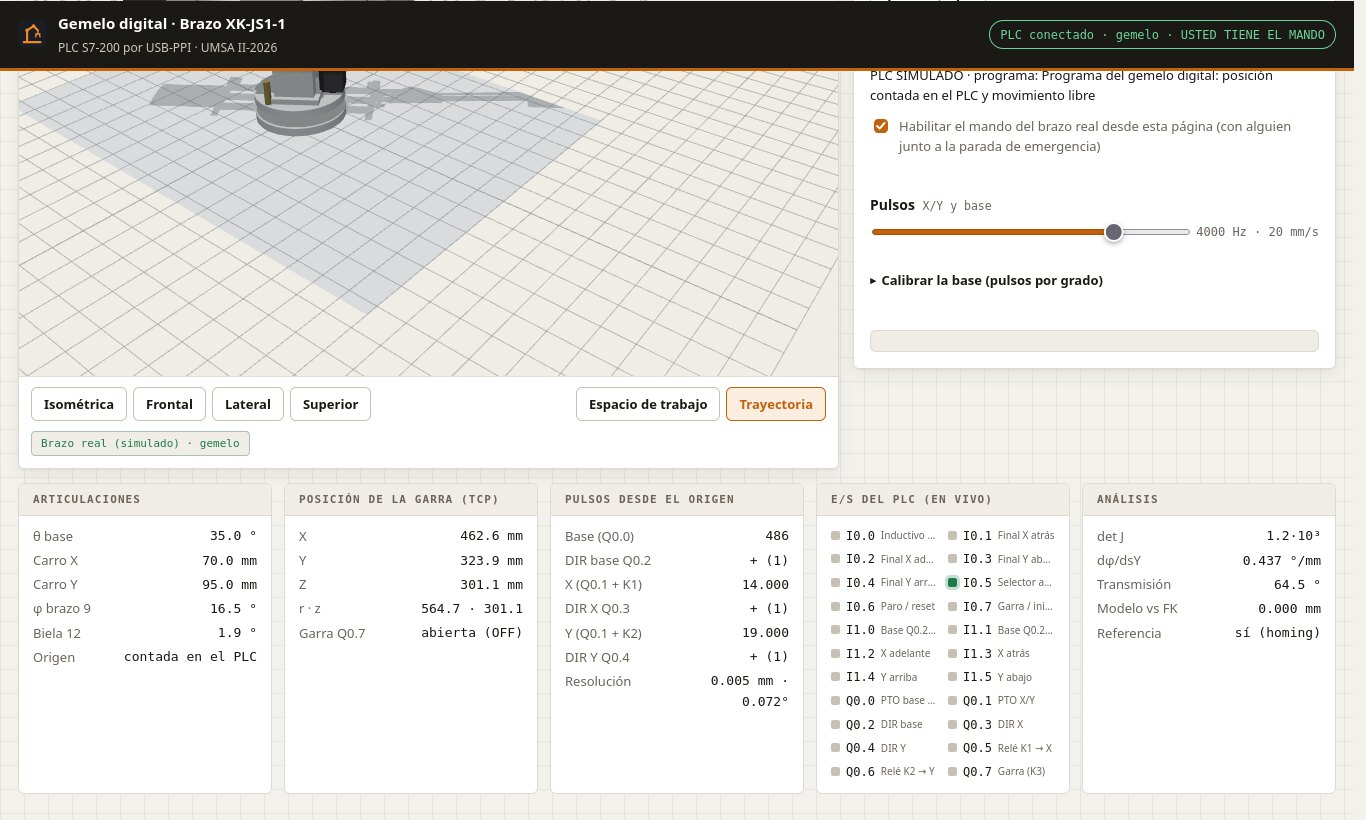
\includegraphics[width=\linewidth, trim=0 0 0 440, clip]{img/local_conexion_abajo.jpg}
\caption{Telemetría, debajo del visor: articulaciones, posición de la garra, pulsos desde el origen, entradas y salidas reales del PLC (I0.0--I1.5 y Q0.0--Q0.7) y análisis (determinante del jacobiano, transmisión y referencia).}
\end{figure}

\begin{figure}[H]
\centering
\captura{\linewidth}{img/local_cartesiano.jpg}{
  \node[marca] at (0.61,0.80) {1};
  \node[marca] at (0.61,0.66) {2};
  \node[marca] at (0.61,0.545) {3};
  \node[marca] at (0.61,0.47) {4};
}
\caption{Pestaña \emph{Cartesiano}, con un punto fuera del alcance.}
\end{figure}
\begin{enumerate}[label=\num{\arabic*}, leftmargin=9mm]
\item Ayuda: el origen está en el eje de giro sobre la mesa, X apunta al sensor inductivo ($\theta=0$) y Z hacia arriba.
\item \textbf{X, Y, Z} de la garra en mm.
\item \textbf{Mover} calcula la cinemática inversa y manda las posiciones de los ejes. \textbf{Usar posición actual} copia la posición de la garra en los campos.
\item Si el punto no se alcanza, la página lo dice y \textbf{propone el punto alcanzable más cercano}; \emph{Usar ese punto} lo copia en los campos.
\end{enumerate}
\nota{\textbf{Por qué muchos puntos salen \emph{inalcanzables}.} Los dos carros se mueven en diagonal y la zona que barre la garra es una franja estrecha. Justo después del homing (X = Y = 0) el brazo está en una esquina de esa franja: desde ahí, por ejemplo, subir o bajar la garra en línea recta pide que el carro X retroceda por debajo de 0. Lo práctico es partir de \emph{Usar posición actual} y cambiar los valores de a poco, o mover primero con la pestaña \emph{Articular}. Con el brazo real, X e Y comparten el tren de pulsos, así que la trayectoria no es recta: los dos carros avanzan juntos y el de menor recorrido se detiene antes.}

\begin{figure}[H]
\centering
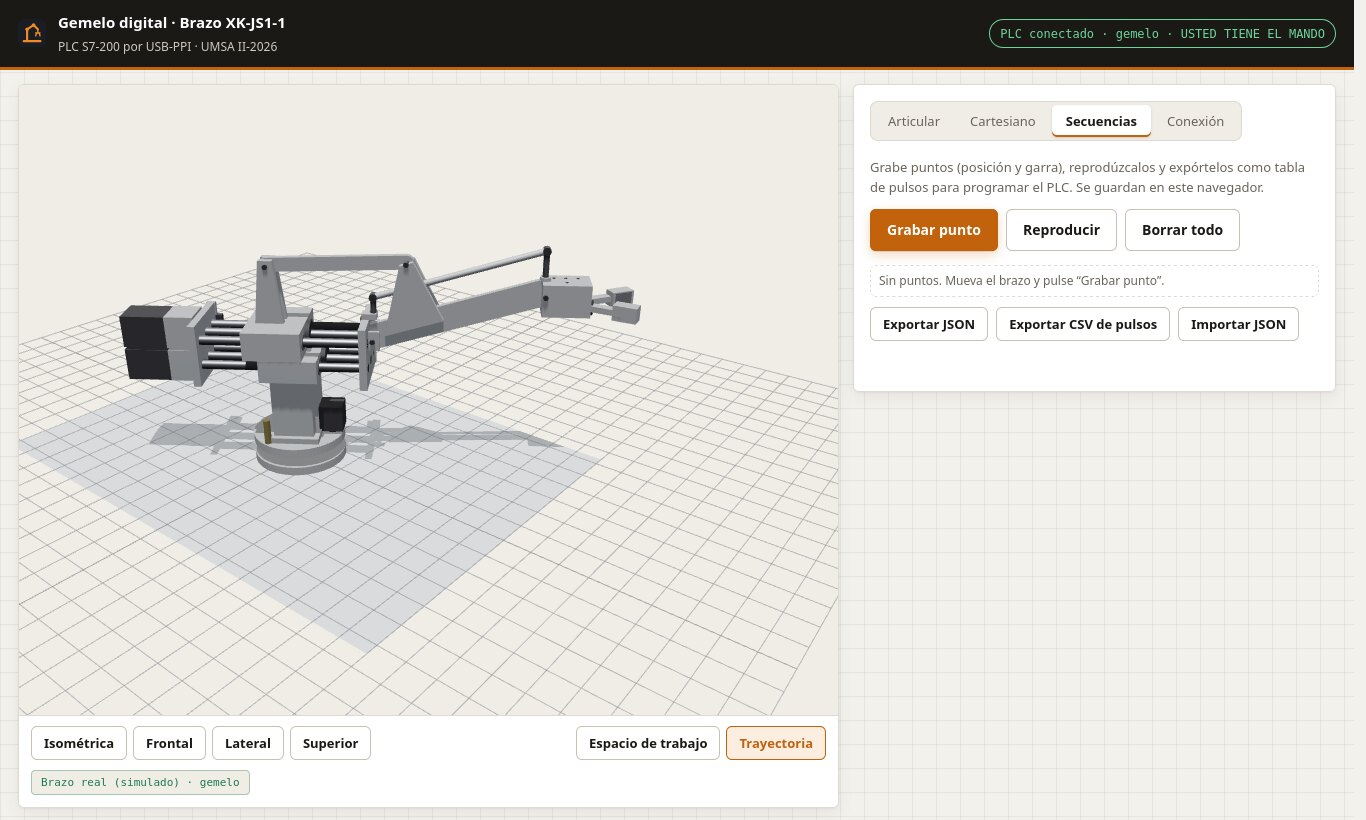
\includegraphics[width=0.9\linewidth]{img/local_secuencias.jpg}
\caption{Pestaña \emph{Secuencias}: \emph{Grabar punto} guarda la posición y el estado de la garra; \emph{Reproducir} los recorre esperando que el PLC termine cada uno; los puntos se exportan como JSON o como tabla CSV de pulsos para programar el PLC.}
\end{figure}

\subsection{Primer uso con el programa del gemelo}
\begin{enumerate}
\item Selector del panel en \emph{automático}.
\item Pestaña \emph{Conexión}: marque \emph{Habilitar el mando} y confirme.
\item Pestaña \emph{Articular}: \textbf{Homing}. El orden es Y abajo hasta I0.3, X atrás hasta I0.1, abrir la garra y girar la base hasta I0.0. Al terminar desaparece el aviso \emph{Sin referencia}.
\item Mueva con \emph{Articular}, \emph{Cartesiano} o \emph{Secuencias}.
\item \textbf{Detener} corta el movimiento; la posición deja de ser exacta y el PLC pide un nuevo homing.
\end{enumerate}

\subsection{Con el programa anterior (perfil \emph{cargado})}
Ese programa no lleva la cuenta de la posición y solo ejecuta sus secuencias fijas, así que la página es sobre todo un \textbf{monitor}: con el selector en \emph{manual} se mueve el brazo con el panel y el modelo lo sigue con una posición estimada, que se corrige en los finales de carrera y en el inductivo. Con el mando habilitado aparecen los botones \emph{Iniciar} (igual que I0.7: homing sin referencia, luego secuencia 1 y 2), \emph{Detener}, \emph{Paro de emergencia (PC)} y \emph{Rearmar}. El homing exige el selector en \emph{automático}; en \emph{manual} ese programa usa el inicio solo para la garra, y la app lo avisa.

\subsection{Calibrar la base}\label{sec:calibrar}
La reducción de la base no se conocía; hoy está calibrada en 190,3 pulsos por grado (\codigo{calibracion.json}). Para repetirla:
\begin{enumerate}
\item Haga el homing: la base queda en el sensor inductivo ($\theta = 0$).
\item Gire la base (con el panel o con la página) y mida el ángulo con un transportador.
\item En \emph{Conexión $\rightarrow$ Calibrar la base}, escriba el ángulo (positivo si giró como con I1.0) y pulse \emph{Calibrar}.
\end{enumerate}

% =====================================================================
\section{Usuarios y contraseñas}\label{sec:usuarios}

Los usuarios se crean \textbf{solo en la PC del laboratorio}, con la herramienta \codigo{usuarios.py} que está junto a la app. Las contraseñas no se muestran al escribirlas y se guardan cifradas (PBKDF2) en \codigo{usuarios.json}; ese archivo no se sube a GitHub. Los cambios valen al momento, sin reiniciar la app.

\begin{center}\small
\begin{tabularx}{\linewidth}{>{\raggedright}p{8.6cm} >{\raggedright\arraybackslash}X}
\toprule
\textbf{Comando} (en la carpeta de la app) & \textbf{Qué hace}\\
\midrule
\codigo{python3 usuarios.py listar} & lista los usuarios y su rol\\
\codigo{python3 usuarios.py agregar ana -{}-rol operador} & crea un operador (pide la contraseña dos veces)\\
\codigo{python3 usuarios.py agregar visita -{}-rol observador} & crea un observador\\
\codigo{python3 usuarios.py clave visita} & cambia la contraseña\\
\codigo{python3 usuarios.py rol visita operador} & cambia el rol\\
\codigo{python3 usuarios.py quitar visita} & borra el usuario\\
\bottomrule
\end{tabularx}
\end{center}

Ejemplo de \codigo{listar}:
\begin{lstlisting}
GABGOM               operador
operador_1           operador
visita               observador
\end{lstlisting}

\begin{center}\small
\begin{tabularx}{\linewidth}{>{\raggedright}p{2.6cm} >{\raggedright\arraybackslash}X}
\toprule
\textbf{Rol} & \textbf{Qué puede hacer}\\
\midrule
observador & Ver el brazo en vivo: modelo 3D, posición, entradas y salidas. No puede mover, tomar el mando ni dar paro.\\
operador & Todo lo anterior, más tomar el mando y mover el brazo. Un solo operador tiene el mando a la vez; los demás ven quién lo tiene y \textbf{pueden dar paro}. El mando se suelta al desmarcar la casilla, al pulsar \emph{Salir} o cuando vence la sesión (8 h sin uso).\\
\bottomrule
\end{tabularx}
\end{center}

\begin{itemize}
\item La contraseña debe tener al menos 8 caracteres.
\item El nombre de usuario distingue mayúsculas: \codigo{visita} no es \codigo{VISITA}.
\item Tras 5 contraseñas erradas desde un mismo equipo, ese equipo espera 60 s.
\item Si alguien olvida su contraseña, se le pone una nueva con \codigo{clave}; no hay forma de leer la anterior.
\end{itemize}

% =====================================================================
\section{Guía visual: el acceso remoto}\label{sec:remoto}

\subsection{Conectarse desde un celular u otra PC}
\begin{enumerate}
\item En la PC del laboratorio, arranque la app en modo red: menú \emph{Gemelo digital del brazo (red local)} o \codigo{./iniciar\_gemelo.sh -{}-red}. Para probar sin brazo, use \emph{(red local, simulado)}.
\item Anote la dirección que muestra la terminal, por ejemplo \codigo{https://192.168.1.37:8443/}. Si la PC cambia de red, la dirección cambia; la app siempre muestra la actual al arrancar. (Las direcciones \codigo{172.16.\dots} y \codigo{192.168.7.\dots} de esa PC son de la máquina virtual y no sirven.)
\item Conecte el celular \textbf{al mismo Wi-Fi o router} que la PC del laboratorio. Con datos móviles no funciona.
\item Escriba la dirección en el navegador del celular, \textbf{con \codigo{https://} y con \codigo{:8443}}.
\item La primera vez el navegador avisa que la conexión no es privada: el certificado es propio del laboratorio. Pulse \emph{Avanzado $\rightarrow$ Continuar}.
\item Ingrese con su usuario y contraseña.
\end{enumerate}

\begin{figure}[H]
\centering
\begin{minipage}[t]{0.31\linewidth}\centering
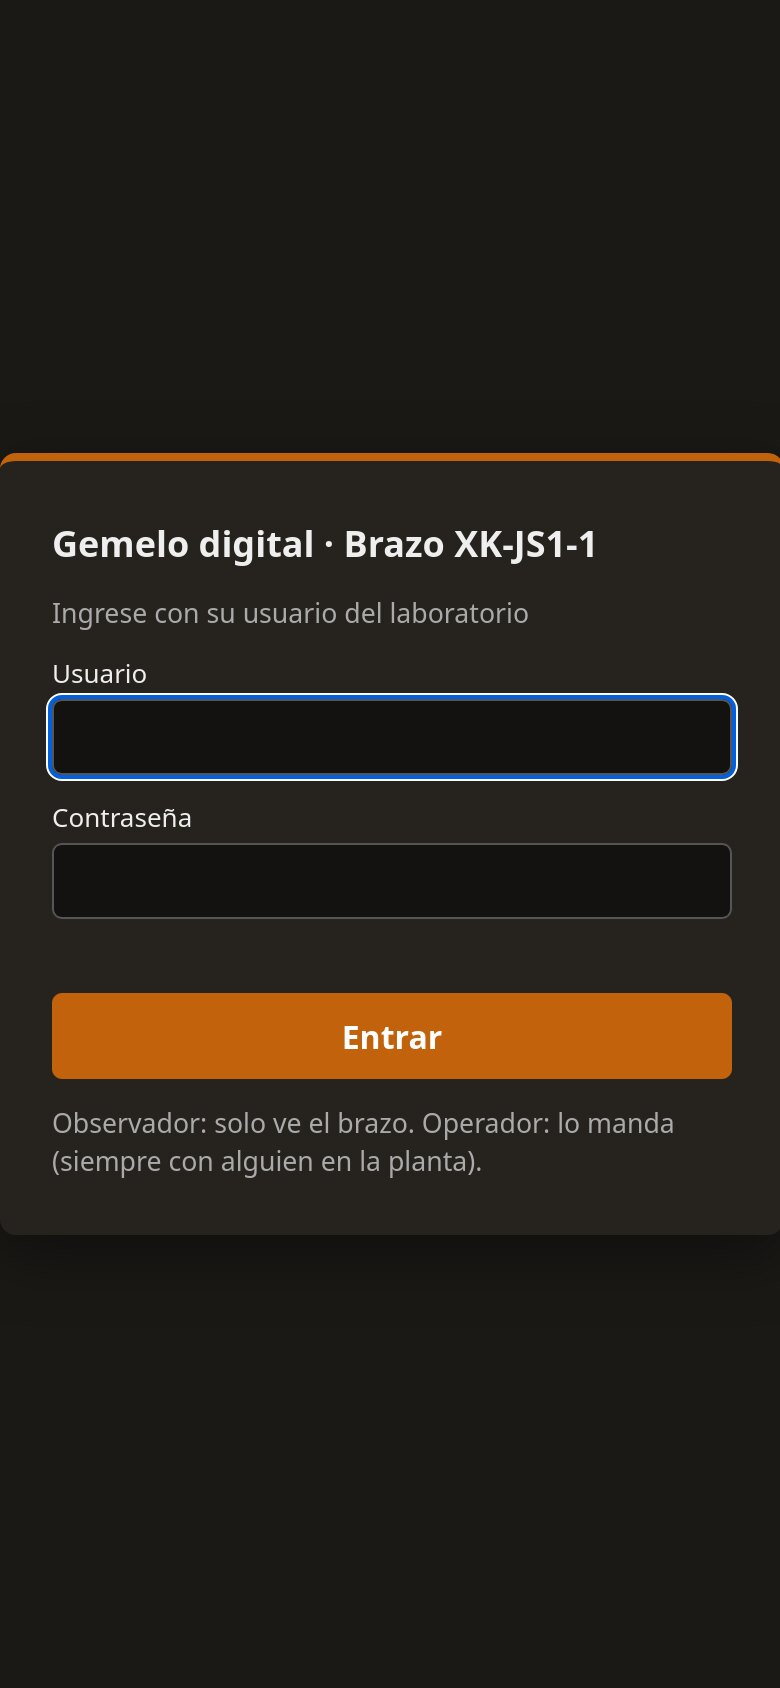
\includegraphics[width=\linewidth]{img/remoto_login.jpg}\\[2pt]
{\small (a) ingreso}
\end{minipage}\hfill
\begin{minipage}[t]{0.31\linewidth}\centering
\captura{\linewidth}{img/remoto_observador.jpg}{
  \node[marca] at (0.80,0.955) {1};
  \node[marca] at (0.50,0.905) {2};
  \node[marca] at (0.07,0.03) {3};
}\\[2pt]
{\small (b) observador}
\end{minipage}\hfill
\begin{minipage}[t]{0.31\linewidth}\centering
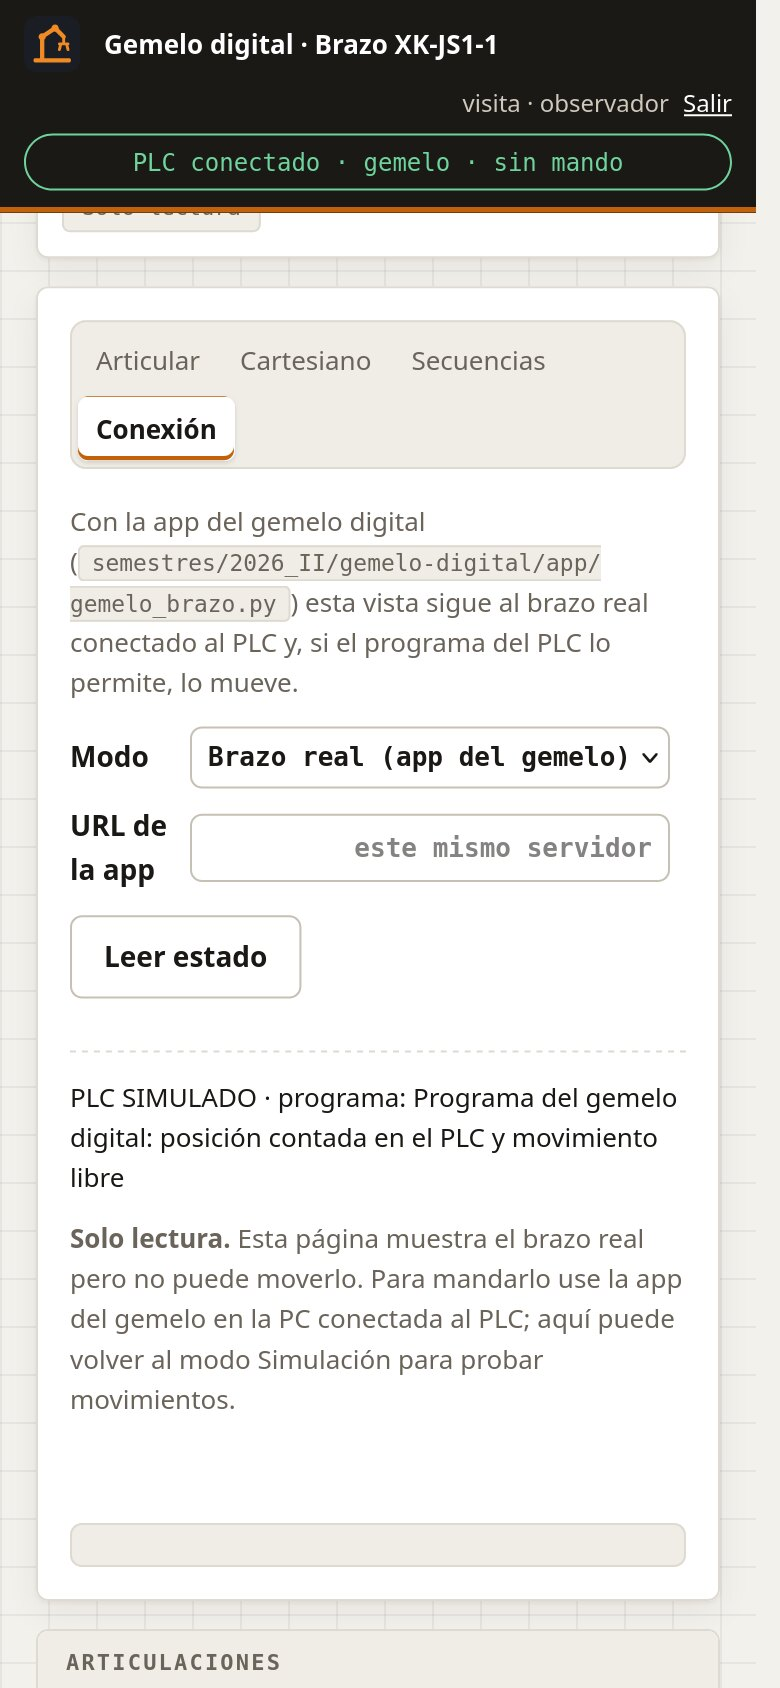
\includegraphics[width=\linewidth]{img/remoto_observador_conexion.jpg}\\[2pt]
{\small (c) observador, pestaña Conexión}
\end{minipage}
\caption{Acceso remoto desde un celular como \textbf{observador}.}
\end{figure}
\begin{enumerate}[label=\num{\arabic*}, leftmargin=9mm]
\item Usuario y rol con que se ingresó, y \emph{Salir} para cerrar la sesión.
\item Estado: PLC conectado, programa y quién tiene el mando.
\item Indicador \emph{Solo lectura}. Los controles de movimiento aparecen bloqueados y la pestaña \emph{Conexión} explica que este usuario solo puede ver. Si igual intenta mandar, la app lo rechaza y lo anota en el registro.
\end{enumerate}

\begin{figure}[H]
\centering
\begin{minipage}[t]{0.31\linewidth}\centering
\captura{\linewidth}{img/remoto_operador_conexion_antes.jpg}{
  \node[marca] at (0.05,0.34) {1};
}\\[2pt]
{\small (a) operador, sin mando}
\end{minipage}\hfill
\begin{minipage}[t]{0.31\linewidth}\centering
\captura{\linewidth}{img/remoto_operador_conexion.jpg}{
  \node[marca] at (0.06,0.905) {2};
  \node[marca] at (0.05,0.40) {3};
}\\[2pt]
{\small (b) mando tomado}
\end{minipage}\hfill
\begin{minipage}[t]{0.31\linewidth}\centering
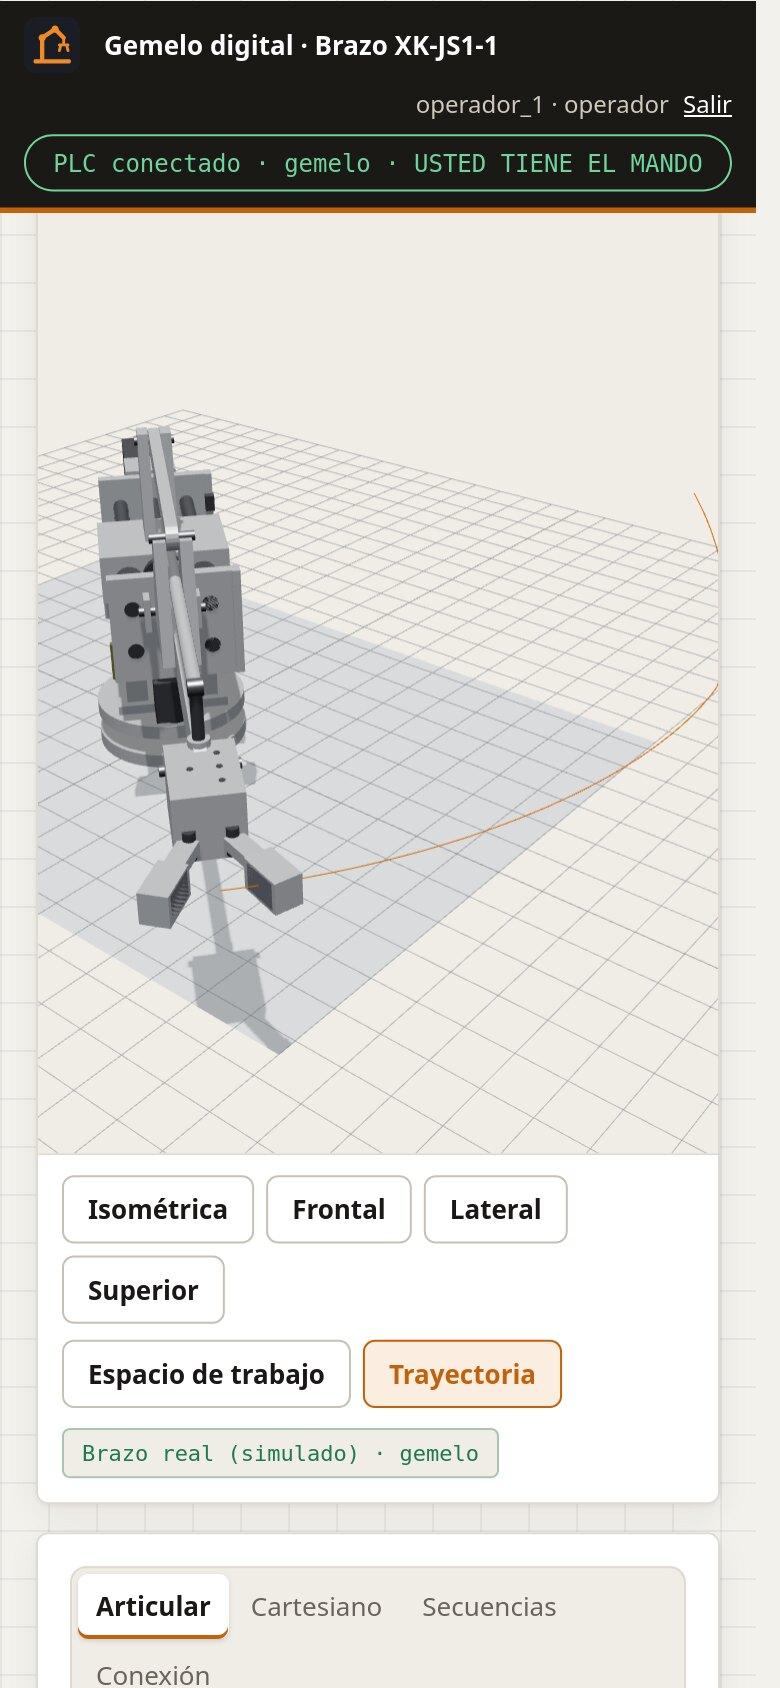
\includegraphics[width=\linewidth]{img/remoto_operador_mueve.jpg}\\[2pt]
{\small (c) el brazo se movió}
\end{minipage}
\caption{Acceso remoto como \textbf{operador}.}
\end{figure}
\begin{enumerate}[label=\num{\arabic*}, leftmargin=9mm]
\item Al ingresar, el operador \textbf{no} tiene el mando: la casilla \emph{Habilitar el mando} está vacía y la página muestra \emph{Mando desde la PC deshabilitado}.
\item Al marcar la casilla y confirmar, el estado pasa a \emph{USTED TIENE EL MANDO}.
\item Desde ahí usa las pestañas \emph{Articular}, \emph{Cartesiano} y \emph{Secuencias} igual que en la app local (sección \ref{sec:local}).
\end{enumerate}

\begin{figure}[H]
\centering
\captura{\linewidth}{img/remoto_observador_pc.jpg}{
  \node[marca] at (0.70,0.965) {1};
  \node[marca] at (0.61,0.51) {2};
  \node[marca] at (0.275,0.048) {3};
}
\caption{Un observador desde una PC mientras el operador \codigo{operador\_1} tiene el mando.}
\end{figure}
\begin{enumerate}[label=\num{\arabic*}, leftmargin=9mm]
\item \emph{mando: operador\_1}: todos ven quién está mandando.
\item Mensaje para el observador: ve el brazo en vivo pero no puede moverlo.
\item \emph{Solo lectura}. Otro \emph{operador} vería aquí \emph{Mando en uso por operador\_1: usted solo puede dar paro}.
\end{enumerate}

\subsection{Comprobar qué hace cada usuario}
En la PC del laboratorio, el registro muestra en vivo los ingresos y las órdenes:
\begin{lstlisting}
tail -f registro_gemelo.log
\end{lstlisting}
\begin{lstlisting}
01:05:58 ingreso de operador_1 (operador) desde 192.168.1.9
01:05:59 ingreso de visita (observador) desde 192.168.1.20
01:05:59 RECHAZADO /api/orden/mover de visita (observador): solo puede ver
01:05:59 mando desde la PC HABILITADO (operador_1)
01:05:59 orden homing  (operador_1)
01:06:05 RECHAZADO /api/orden/mover de operador_1: falta hacer homing
01:06:20 orden mover {"theta": 10, "sX": 20, "sY": 20} (operador_1)
\end{lstlisting}
Las órdenes dadas en la PC del laboratorio aparecen como \codigo{(local)}.

\subsection{Seguridad del acceso remoto}
\begin{itemize}
\item La conexión va cifrada (HTTPS) con un certificado propio del laboratorio.
\item Las órdenes solo se aceptan desde la propia página de la app, no desde otros sitios web.
\item La sesión vence a las 8 h sin uso; \emph{Salir} la cierra al momento y suelta el mando.
\end{itemize}
\aviso{El acceso funciona solo dentro de la red local. Para usarlo desde fuera haría falta un túnel o una VPN (Tailscale es gratuito). Siempre debe haber alguien junto a la seta de emergencia cuando un operador tiene el mando.}

\subsection{La página pública}
La página publicada en internet (\url{https://brazo-4gdl-gemelo-digital.pages.dev}) sirve para estudiar y simular el brazo. Abierta en la misma PC del laboratorio, puede además \emph{ver} el brazo real (pestaña \emph{Conexión}, modo \emph{Brazo real}, URL \codigo{http://localhost:8050}), pero nunca mandarlo: para mandar se usa la app local o el acceso remoto con usuario.

% =====================================================================
\section{Cargar el programa del gemelo en el PLC}
\aviso{Cargar un programa reemplaza el que tiene el PLC. El programa anterior quedó respaldado en \codigo{ETN 1034/respaldo\_vm/programa\_plc\_cargado\_20261026.mwp} (también como \codigo{proyecto1\_abierto.awl}). Para volver a él, se carga ese archivo de la misma forma.}
\begin{enumerate}
\item Cierre la app. En la ventana de la VM, menú \emph{Dispositivos $\rightarrow$ USB}, \textbf{marque} \emph{USB2.0-Serial} para pasar el cable a Windows.
\item En Micro/WIN, \emph{Archivo $\rightarrow$ Abrir}:
\begin{lstlisting}
\\vboxsvr\MIS_COSAS\ETN\ETN 1034\GIT_BRAZO\Brazo-4GDL-gemelo-digital\
  semestres\2026_II\gemelo-digital\plc\brazo_gemelo.mwp
\end{lstlisting}
Si falta el \codigo{.mwp}, cree un proyecto nuevo e importe \codigo{brazo\_gemelo.awl}.
\item \emph{CPU $\rightarrow$ Tipo $\rightarrow$ Leer CPU}; luego \emph{CPU $\rightarrow$ Compilar todo}: debe decir \emph{Total errores: 0}.
\item \emph{Archivo $\rightarrow$ Cargar en CPU}. Si se carga también el bloque de sistema, el PLC queda en la dirección PPI 2 a 9,6 kbit/s (así está hoy); la app lo encuentra igual.
\item Pase el PLC a RUN, devuelva el cable a Linux (desmarque \emph{USB2.0-Serial}) y arranque la app: debe decir \codigo{perfil "gemelo"}.
\item \textbf{Primera prueba}, a baja velocidad y con alguien en la seta: mueva cada eje con el panel (selector en manual) y verifique que el modelo lo sigue y que los finales cortan; luego homing desde la página (selector en automático) y movimientos cortos comparando con una regla.
\end{enumerate}

% =====================================================================
\section{Solución de problemas}
\begin{center}\small
\begin{longtable}{>{\raggedright}p{5.6cm} >{\raggedright\arraybackslash}p{10.2cm}}
\toprule
\textbf{Síntoma} & \textbf{Qué hacer}\\
\midrule
\endhead
\multicolumn{2}{@{}l}{\textbf{Conexión con el PLC}}\\
\codigo{no responde ningún PLC en /dev/ttyUSB0} & PLC apagado, cable desconectado, o la VM tomó el USB (desmárquelo en \emph{Dispositivos $\rightarrow$ USB}). Pruebe \codigo{ls /dev/serial/by-id/}.\\
\codigo{Permission denied: /dev/ttyUSB0} & El usuario no está en el grupo \codigo{dialout} (sección 3).\\
\emph{Sin conexión con el PLC} en la página & La app perdió el cable; reintenta sola cada 2 s y vuelve a buscar la dirección y la velocidad. Mire la terminal.\\
Micro/WIN no se comunica & El cable está en Linux: cierre la app y pase el USB a la VM.\\
\multicolumn{2}{@{}l}{\textbf{Acceso remoto}}\\
El celular no abre la página & 1) Use \codigo{https://} (con \codigo{http://} no carga) y el puerto \codigo{:8443}. 2) No use \codigo{localhost}: esa dirección solo sirve en la PC del laboratorio. 3) El celular debe estar en el mismo Wi-Fi (su IP empieza igual que la de la PC, por ejemplo \codigo{192.168.1.}). 4) Redes de invitados o con \emph{aislamiento de AP} no dejan hablar a los equipos entre sí: use la red principal o el hotspot del celular. 5) Si la PC tiene cortafuegos: \codigo{sudo ufw allow 8443/tcp}.\\
\emph{La conexión no es privada} & Es normal la primera vez: \emph{Avanzado $\rightarrow$ Continuar}.\\
\emph{Usuario o contraseña incorrectos} & El nombre distingue mayúsculas. Ponga una contraseña nueva con \codigo{python3 usuarios.py clave NOMBRE}.\\
\emph{Espere \dots{} s} al ingresar & Hubo 5 intentos fallidos: espere 60 s.\\
\emph{su usuario es observador} & Ese usuario solo puede ver. Cámbielo con \codigo{python3 usuarios.py rol NOMBRE operador}.\\
\emph{Mando en uso por \dots} & Otro operador tiene el mando: puede dar paro, pero no mover hasta que lo suelte.\\
\emph{el mando desde la PC está deshabilitado} & Marque \emph{Habilitar el mando} en la pestaña \emph{Conexión}.\\
\multicolumn{2}{@{}l}{\textbf{Movimiento}}\\
\emph{Selector en manual} & Gire el selector del panel a automático para mandar desde la PC o un celular.\\
\emph{falta hacer homing} & Use \emph{Homing}.\\
\emph{Inalcanzable} en \emph{Cartesiano} & El punto está fuera de la franja que alcanza la garra: use \emph{Usar ese punto} o cambie los valores de a poco desde la posición actual.\\
\emph{destino fuera del recorrido} & El punto pedido sale de 0--170 mm en X/Y o del giro permitido.\\
\emph{watchdog} & La página o la app dejaron de responder durante un movimiento: vuelva a hacer homing.\\
El modelo no coincide con el brazo & Haga homing. Con el programa anterior la posición es estimada y se corrige en los finales de carrera.\\
\bottomrule
\end{longtable}
\end{center}

% =====================================================================
\section{Referencia: memoria del programa del gemelo}
\begin{center}\small
\begin{longtable}{@{}p{4.3cm}p{2.1cm}p{9.6cm}@{}}
\toprule
\textbf{Dirección} & \textbf{Quién escribe} & \textbf{Contenido}\\
\midrule
VB1100 & PC & orden: 1 homing, 2 mover, 3 paro, 4 cerrar garra, 5 abrir garra\\
VB1101 & PC & secuencia: el PLC ejecuta la orden cuando cambia\\
VW1102 & PC & latido (watchdog de 2 s durante un movimiento pedido por la PC)\\
VD1104 / VD1108 / VD1112 & PC & pulsos relativos de base / X / Y (con signo)\\
VW1116 / VW1118 & PC & ciclo del tren de pulsos X/Y y base [µs] (200--2000 y 250--4000)\\
VB1120 & PLC & estado: 0 reposo, 1 homing, 2 moviendo\\
VB1121 & PLC & eco de la secuencia\\
VB1122 & PLC & bits: .0 referenciado, .1 remoto (I0.5), .2 PTO0 y .3 PTO1 ocupados, .4 posición incierta, .5 watchdog\\
VB1123 & PLC & error: 1 ocupado, 2 fuera de recorrido, 3 watchdog, 4 sin homing, 5 orden desconocida, 6 paro\\
VD1124 / VD1128 / VD1132 & PLC & posición de base / X / Y [pulsos]\\
VW1136 & PLC & paso de la máquina de estados\\
VB1138 / VB1139 / VB1140 & PLC & copia de IB0 / IB1 / QB0\\
VB1141 & PLC & firma 16\#47 (la app reconoce así el programa)\\
VD1144 / VD1148 / VD1152 & PLC & tramo en curso de base / X / Y [pulsos]\\
\bottomrule
\end{longtable}
\end{center}
Sentidos: X positivo con Q0.3 = 0 (adelante), Y positivo con Q0.4 = 0 (arriba), base positiva con Q0.2 = 0 (SUPUESTO). Recorridos: X e Y de 0 a 34000 pulsos (170 mm a 0,005 mm/pulso); base $\pm$50000 pulsos (SUPUESTO).

\section{Referencia: memoria del programa anterior}
\begin{center}\small
\begin{tabular}{@{}lll@{}}
\toprule
\textbf{Dirección} & \textbf{Quién escribe} & \textbf{Contenido}\\
\midrule
V104.0 & PC & iniciar (igual que I0.7)\\
V104.1 & PC & paro en automático\\
V104.2 & PC & emergencia (enclavada)\\
V104.7 & PC & latido: si no cambia en 5 s el PLC borra VB104\\
V100.3 & PC & rearmar (flanco)\\
V200.0 / .1 / .3 / .7 & PLC & listo / ocupado / falla de homing / referenciado\\
V301.0 / .2 / .4 & PLC & homing / secuencia 1 / secuencia 2 en curso\\
VW320 / VW322 & PLC & paso del automático / del homing\\
\bottomrule
\end{tabular}
\end{center}

\section{Limitaciones y supuestos}
\begin{itemize}
\item El sentido de giro de la base es un \textbf{SUPUESTO}; su reducción se calibró midiendo un ángulo (190,3 pulsos por grado).
\item Los programas dan los pulsos sin rampa: a más de 4--5 kHz los motores pueden perder pasos.
\item Con el PLC a 9,6 kbit/s cada lectura tarda unos 150 ms; el visor interpola entre lecturas.
\item X e Y comparten un solo tren de pulsos (Q0.1 con los relés K1 y K2): las trayectorias cartesianas no son rectas.
\item Los finales de carrera de X e Y cortan el movimiento en el programa del gemelo. La base no tiene finales: su límite es de software ($\pm$50000 pulsos en el PLC y $\pm$175° en la app, SUPUESTO).
\item El acceso remoto llega solo a la red local.
\end{itemize}

\end{document}
